% !TEX root = main.tex
% This file contains the "LLM-as-a-Judge Assessment" subsection,
% converted from Experiments.md.
% Required packages (add to your preamble if not already loaded):
%   \usepackage{booktabs}
%   \usepackage{graphicx}
%   \usepackage{amsmath}
%   \usepackage{amssymb}
%   \usepackage{xcolor}
%   \usepackage{listings}  % only if you want fancy code formatting

\subsection{LLM-as-a-Judge Assessment}
\label{sec:llm-judge}

\paragraph{Protocol.}
To complement the automatic privacy--utility metrics, we conduct a
fine-grained LLM-as-a-Judge evaluation (GPT-4o-mini) on 500 rewrites per
system (1{,}500 in total) for our method and two strong baselines,
\emph{Papillon} and \emph{Prediax}. Given the original question and the
rewritten query, the judge produces (i) flags for four privacy-leak
categories and five utility-issue categories, (ii) any newly
hallucinated sensitive attributes, and (iii) a re-identification risk
score $r\in[0,1]$, a utility score $u\in[0,1]$, and a verdict in
$\{\textsf{good}, \textsf{acceptable}, \textsf{bad}\}$. The four leak
and five utility categories are defined in
Appendix~\ref{app:judge-rubric}.

\paragraph{Aggregate results.}
We observe a clear negative correlation between $r$ and $u$
(Pearson $-0.43$ overall), confirming the expected privacy--utility
tension. Within this tension, our rewrites occupy the most balanced
region of the score space: $11.2\%$ of our samples fall into the
\emph{ideal} high-utility / low-risk quadrant ($u>0.7$ and $r\le 0.5$)
--- comparable to Prediax ($14.8\%$) --- while our \emph{worst-case}
quadrant (low utility and high risk) contains only $3.6\%$ of samples,
less than half of Prediax's $9.0\%$. This suggests that our method
produces fewer catastrophic rewrites than Prediax while remaining more
informative than Papillon.

\begin{figure}[t]
  \centering
  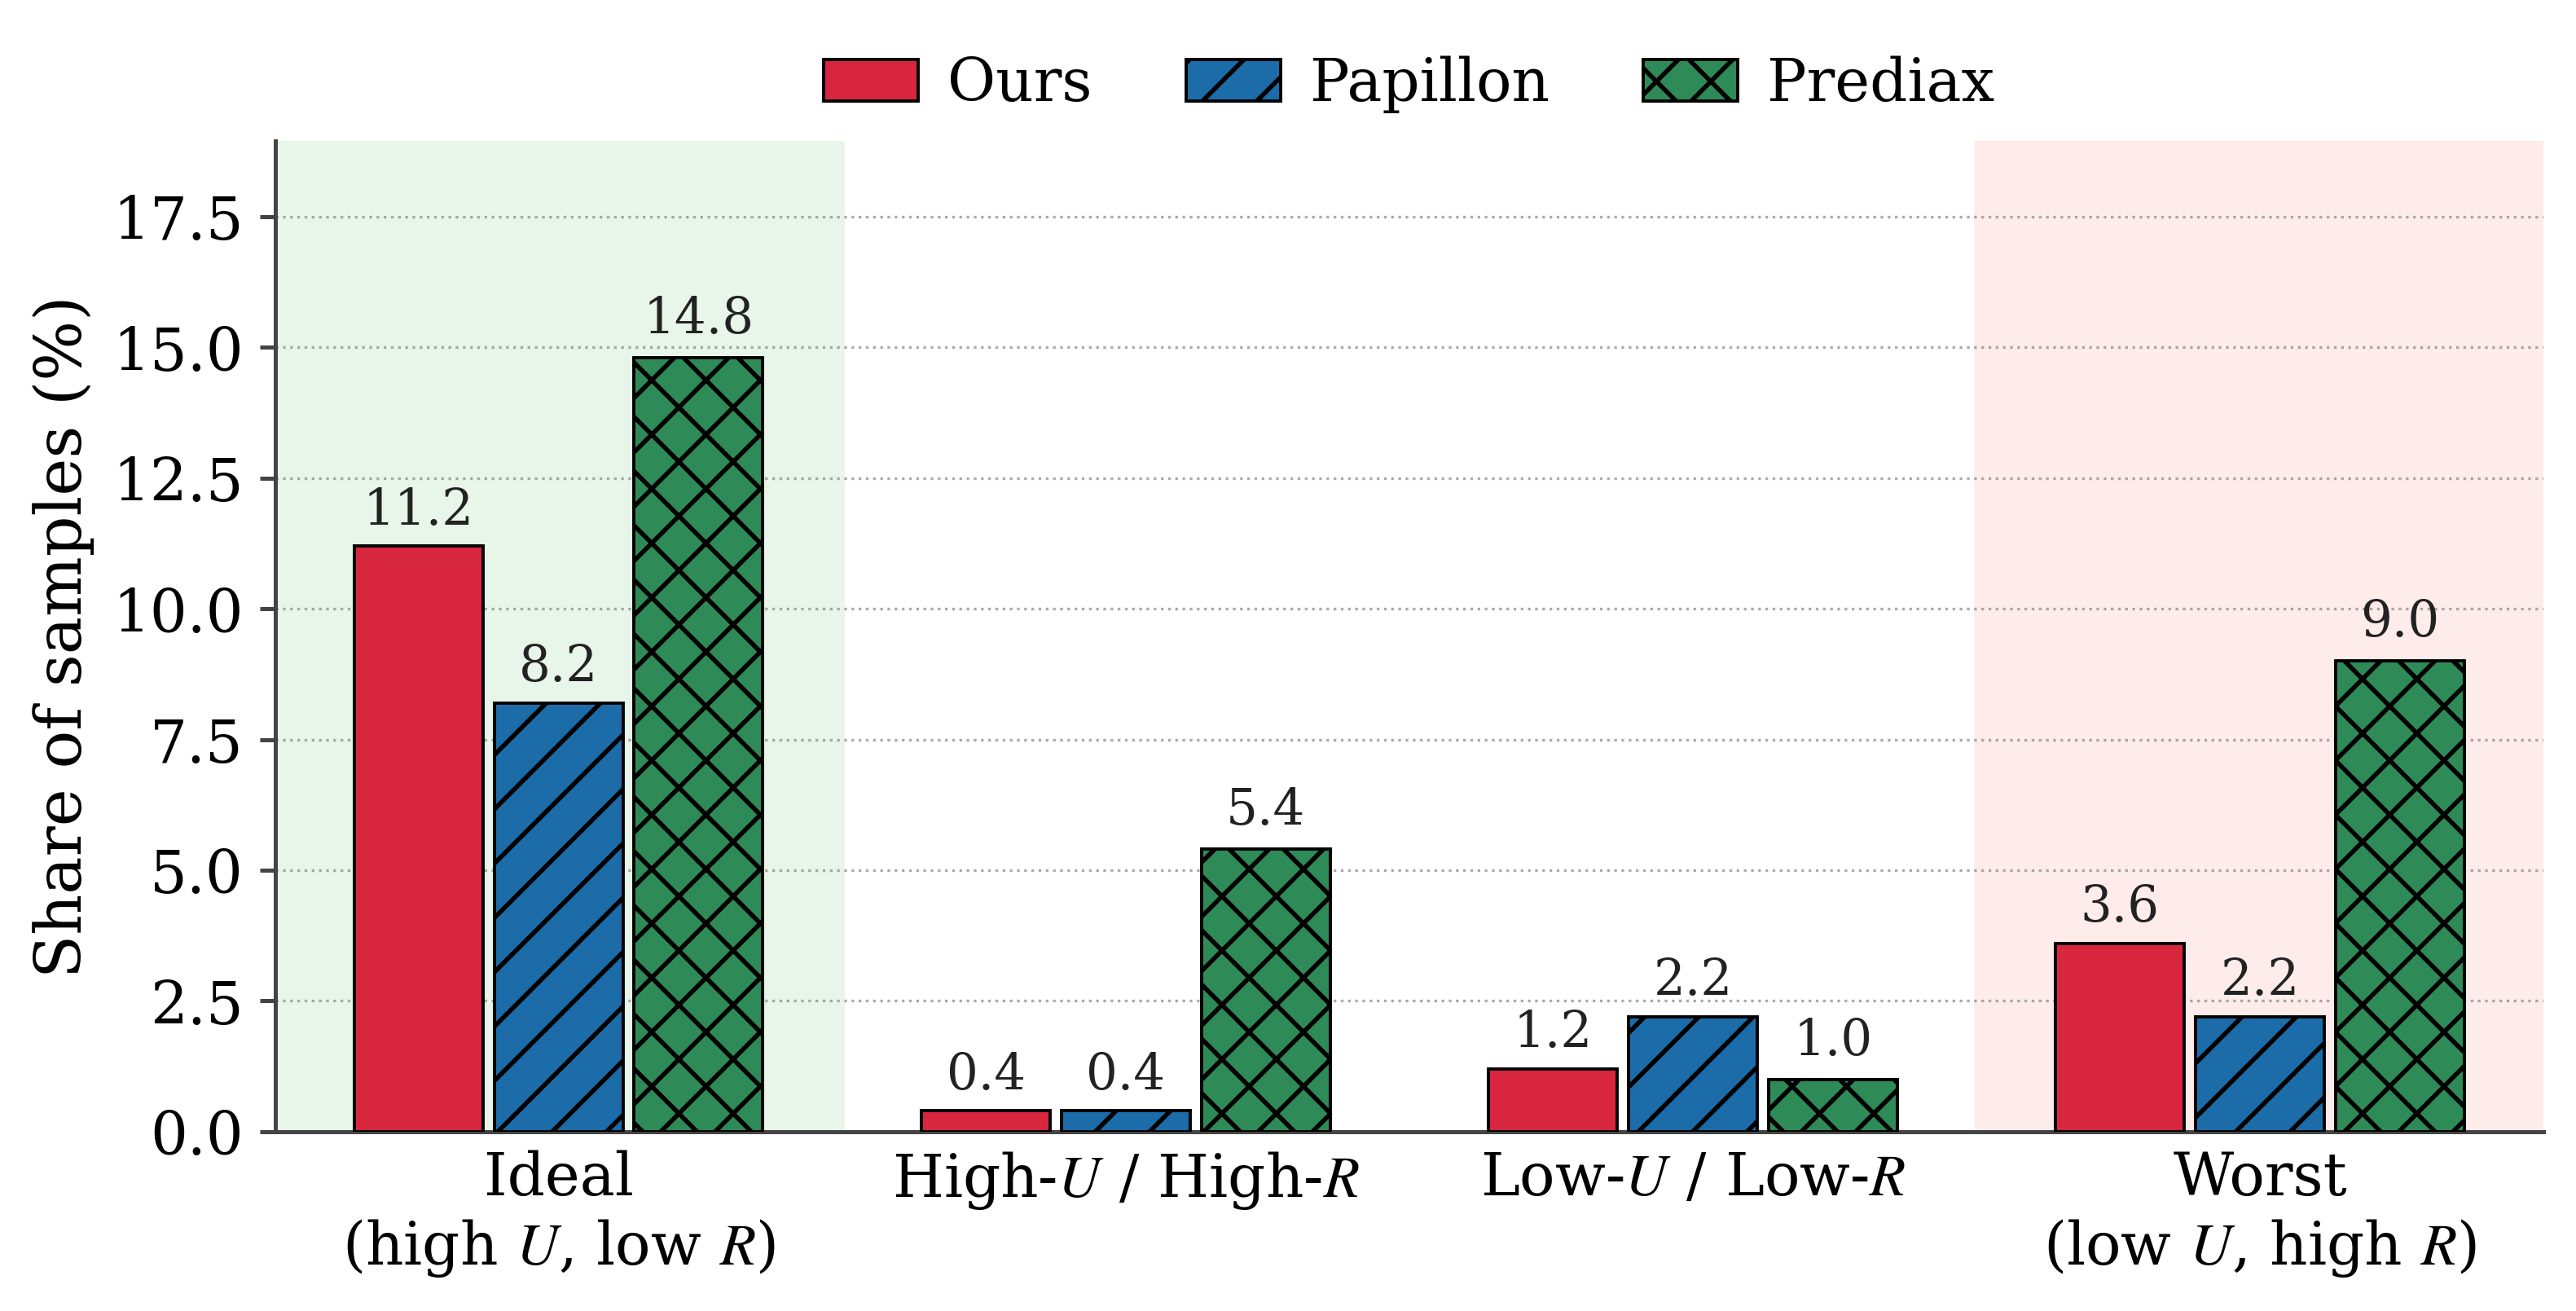
\includegraphics[width=0.85\linewidth]{llm_test_data/results/analysis/08_quadrant_distribution.png}
  \caption{Joint distribution of utility score $u$ and re-identification
  risk score $r$ across the three systems. Our method occupies the
  most balanced region, with relatively few samples in the
  low-utility / high-risk quadrant.}
  \label{fig:quadrant-distribution}
\end{figure}

\paragraph{Privacy-failure mode analysis.}
Breaking the privacy-issue rate down by leak type
(Table~\ref{tab:leaks}) shows that the three systems fail in
qualitatively different ways. Prediax relies heavily on placeholder
substitution (e.g., \texttt{<PERSON>}, \texttt{<DATE\_TIME>}) and
consequently exhibits the highest \texttt{direct\_leak} rate
($51.8\%$ of samples), because non-name tokens such as identifiers,
diagnoses, or device names are left untouched. Papillon performs the
most aggressive paraphrasing and therefore reduces direct leakage to
$15.8\%$, but its rewrites retain enough correlated context to trigger
\texttt{combination\_leak} in $50.8\%$ of samples. Our method sits
between these two regimes, with the lowest \emph{severe} leakage rate
(direct $+$ semantic combined: $25.2\%$, vs.\ $20.0\%$ / $54.4\%$ for
Papillon / Prediax) and the lowest fraction of multi-issue privacy
failures ($4.2\%$ vs.\ $7.2\%$ / $12.2\%$).

\begin{table}[t]
  \centering
  \small
  \caption{Privacy-leak rates (\%) by category. Bold marks the best
  (lowest, except for ``\,$\ge 1$ issue'' / ``\,$\ge 2$ issues'' columns
  where lower is also better) value per column among comparable systems.}
  \label{tab:leaks}
  \begin{tabular}{lcccccc}
    \toprule
    System   & direct        & semantic     & inferential  & combination   & $\ge 1$ issue   & $\ge 2$ issues \\
    \midrule
    Papillon & 15.8          & 4.2          & 12.8         & \textbf{50.8} & 76.4            & 7.2            \\
    Prediax  & 51.8          & 2.6          & 10.6         & 34.6          & 86.2            & 12.2           \\
    \textbf{Ours} & 23.0     & \textbf{2.2} & \textbf{8.0} & 39.6          & \textbf{68.4}   & \textbf{4.2}   \\
    \bottomrule
  \end{tabular}
\end{table}

\paragraph{Utility-failure mode analysis.}
On the utility side, the dominant failure across all systems is
\texttt{lost\_constraint}, which is consistent with the observation
that anonymization tends to drop execution-relevant specifics. Severe
utility failures (\texttt{task\_drift}, \texttt{over\_generalization})
remain rare ($<0.3\%$) but, when they occur, drive the utility score
down to ${\sim}0.20$. Our method exhibits slightly fewer multi-issue
utility failures ($2.2\%$) than the two baselines ($6.8\%$ / $5.4\%$),
indicating that the constraint loss it does incur is typically
confined to a single mild weakening rather than compounding into task
drift.

\paragraph{Hallucinated sensitive content.}
A non-trivial $7.2\%$ of all rewrites introduce sensitive attributes
that are not entailed by the original question
($108 / 1{,}500$ samples, $130$ spans), spanning categories such as
contact identifiers ($11.5\%$ of spans), locations, demographics, and
family or medical context. The rate is comparable across systems
(Papillon $9.2\%$, Ours $6.6\%$, Prediax $5.8\%$), suggesting this is
a general hazard of LLM-driven rewriting and motivates explicit
constraints against attribute hallucination in future work.
